\documentclass[12pt, titlepage]{article}
\usepackage{xcolor} % for different colour comments

%% Comments
\newif\ifcomments\commentstrue

\ifcomments
\newcommand{\authornote}[3]{\textcolor{#1}{[#3 ---#2]}}
\newcommand{\todo}[1]{\textcolor{red}{[TODO: #1]}}
\else
\newcommand{\authornote}[3]{}
\newcommand{\todo}[1]{}
\fi

\newcommand{\wss}[1]{\authornote{magenta}{SS}{#1}}
\newcommand{\ds}[1]{\authornote{blue}{DS}{#1}}

%% Graphics
\usepackage{float}
\usepackage{caption}
\usepackage{graphicx}
\graphicspath{ {Images/} }

\begin{document}

\title{Smart Waiter System Architecture} 
\author{Meraj Patel \#1137491 \\ Pavneet Jauhal \#1149311\\ Shan Perera \#1150394}
\date{\today}
\maketitle

\tableofcontents 

\listoffigures

\listoftables

\begin{table}[H]
\section*{Revision History}
\begin{tabular}{|c|c|}
\hline
\textbf{Date}  & \textbf{Comments} \\ \hline
October 9, 2015 &  first draft. \\ 
\hline
\end{tabular}
\caption{Revision History Table}
\end{table}

\section*{Template}
This document uses Volere Template for its organization.
\pagebreak

\section{Introduction}

\subsection{Purpose}

\subsection{Description}

\subsection{Scope}

\section{Overview}

\section{System Architecture}

\section{Orders}

\subsection{Overview}
Below are key details of ordering component for Smart Waiter application. Detailed architecture review is provided.

\subsection{Ordering Structure}
There are three primary classes used to hold all vital information regarding ordering. These are: MenuCategories, MenuItems and User. Each class purpose and its correlation with each other is explained below.

\subsubsection{MenuCategories Class}
This class purpose is to store menu category information of a restaurant menu. This entails category name, picture and a reference to category items. To do so, there are three main variables used within this class to hold this information: 

\begin{description}
  \item[categoryName:] Stores category name in the form of String
  \item[picURL:] Stores URL of category picture
  \item[categoryItems:] Stores an array of objects that reference MenuItems class
\end{description}


This class is instantiated and called upon when a user successfully scans a barcode. The JSON response acquired from the database is parsed, and information related to menu categories is stored appropriately within this class. The application uses this class to display category information when "Menu Categories" page is spawned (please see section 5.1.1 to view picture).

\subsubsection{MenuItems Class}
This class purpose is to store menu item information of a restaurant menu. This means, item name, price and description. Thee main variables are used within this class to hold this information.

\begin{description}
  \item[itemName:] Stores item name
  \item[itemPrice:] Stores item price
  \item[itemDetail:] Stores description of item
\end{description}

Objects of this class are instantiated from the MenuCategories class. By successfully scanning the barcode and parsing the JSON response, MenuItem objects are instantiated and used to save item details. These objects are held within categoryItems list seen in Menu Categories class. This application uses this class to display item information of a category when "Menu Items" page is spawned (please see section 5.1.2 to view picture). These objects are also used in reference to items the user would like to order. This is thoroughly discussed in the proceeding section.  

\subsubsection{User Class}
User class is used to store menu item a user would like to order. For now, there is only one important variable to consider: 

 \begin{description}
  \item[userItem:] an array that stores objects of MenuItems class. This is used to save menu items a user would like to order.
\end{description}

Only one object is instantiated through the life time of this application. This object represents the user cart of menu items he/she would like to order. This object is called upon when a user decides to add an item to their cart. When this occurs, a copy of the MenuItem object is saved within the userItem variables. This way, there is a list maintained to hold all item a user would like to order. When a user confirms and sends their order, the item information is extracted from userItem list, formatted into a JSON request and send back to the database for further processing. Having this class implemented allows extendibility in the future, as all vital information pertaining to a user can be stored within the class (for example, user settings).  

\subsection{Accounts Structure}



\subsection{Transactions Structure}

\section{User Interface Design}

\subsection{User Interface Design Overview}

\subsubsection{Menu Categories}
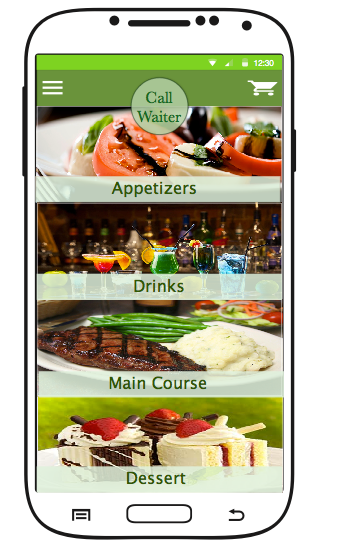
\includegraphics[width=80mm,scale=0.5]{MenuCategories.png}

\subsubsection{Menu Items}
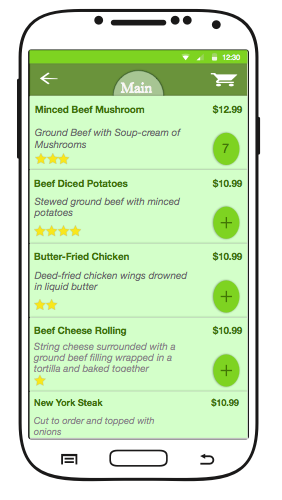
\includegraphics[width=80mm,scale=0.5]{CategoryItems.png}

\subsubsection{Confirm Order}
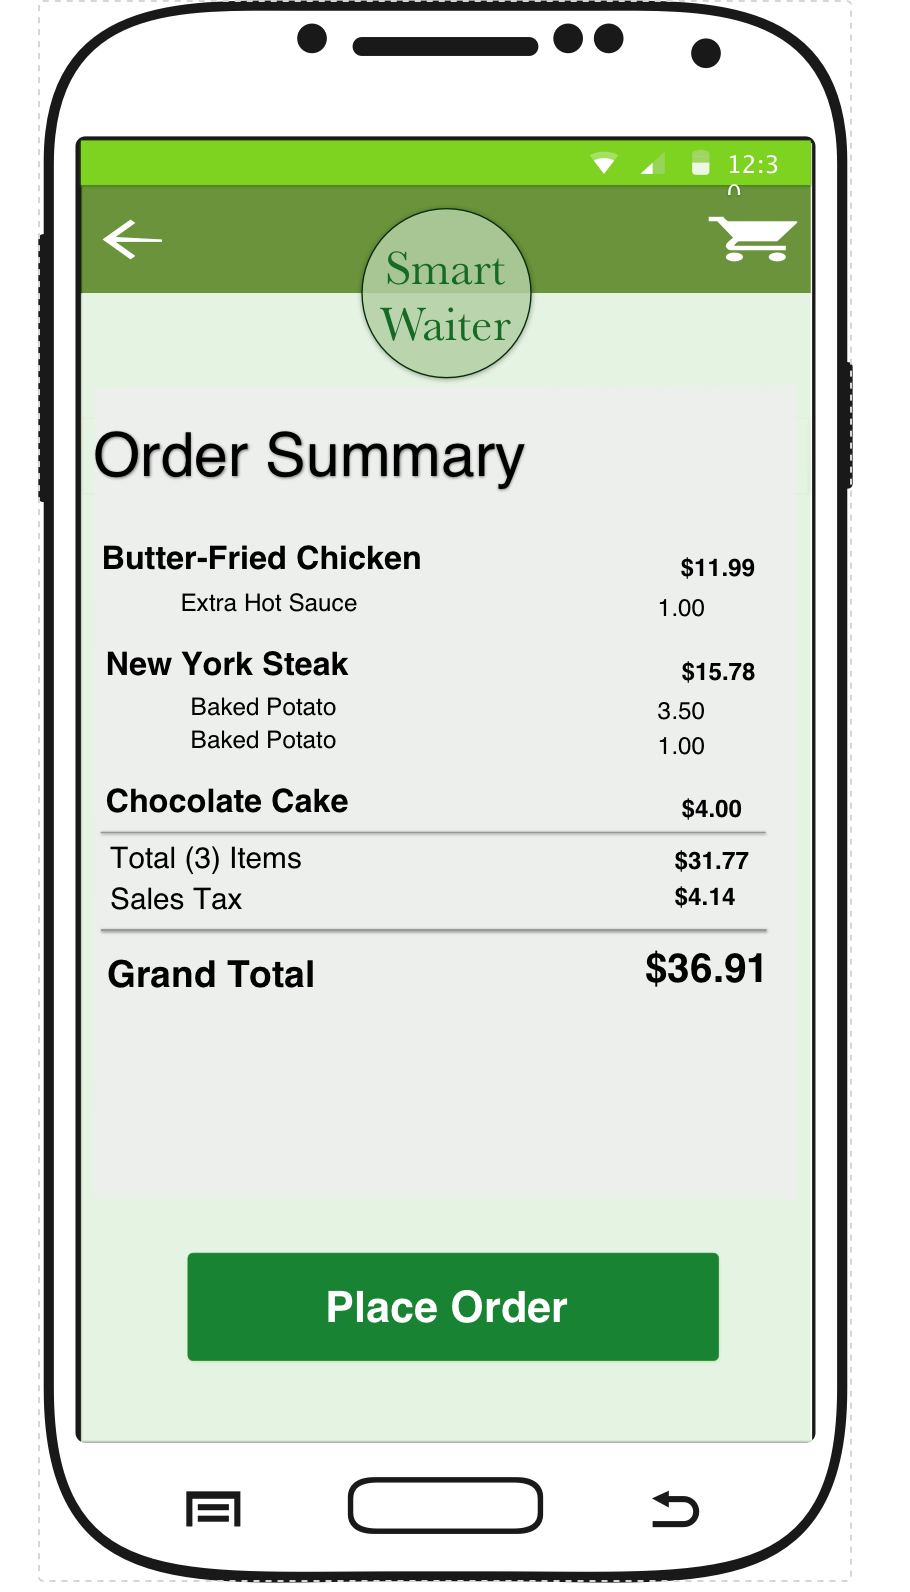
\includegraphics[width=80mm,scale=0.5]{OrderSummary.png}

\subsection{User Interface Navigation Flow}

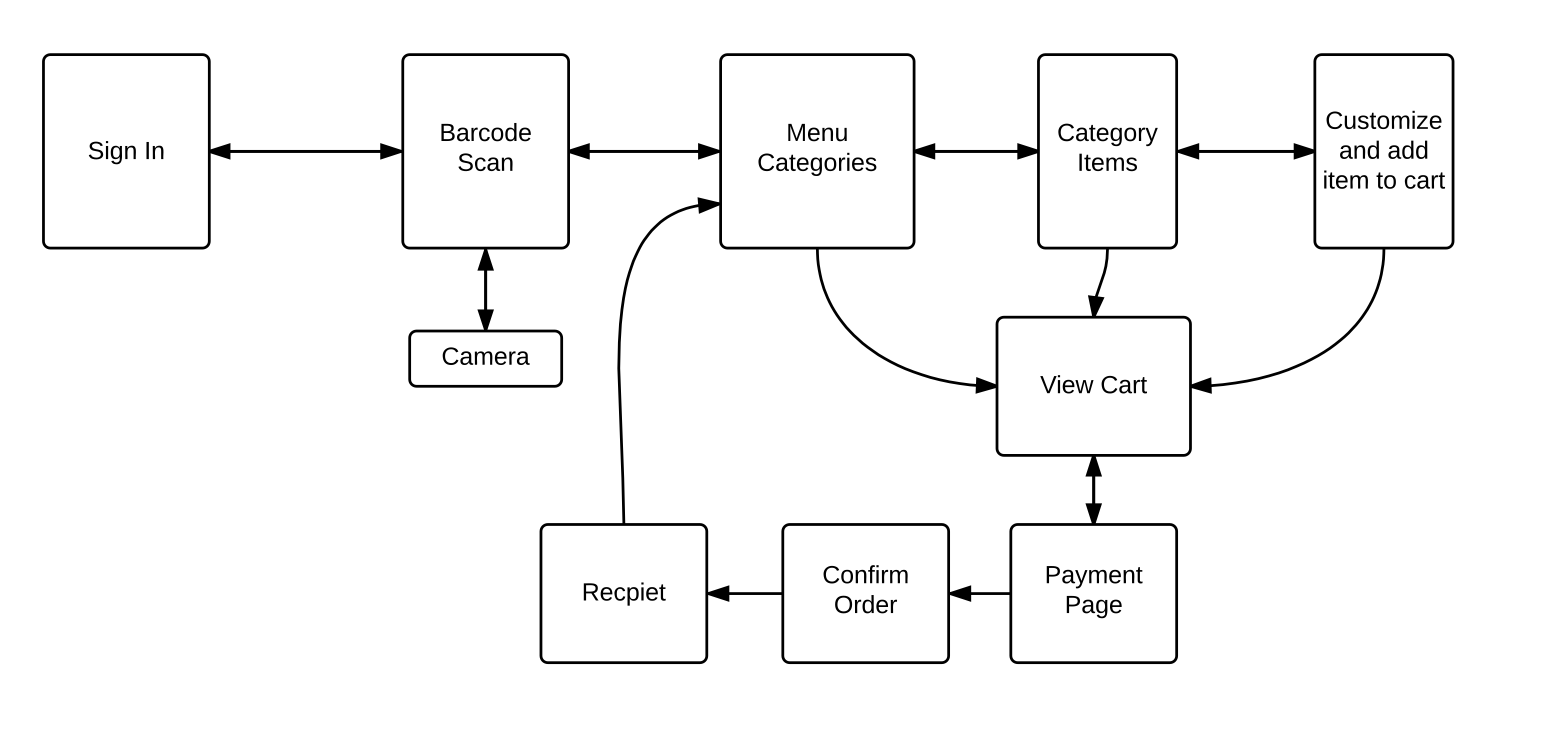
\includegraphics[width=180mm,scale=0.5]{UIProcess.png}

\subsection{Use Cases}

\subsubsection{Sign In Page}
\begin{center}
    \begin{tabular}{ | l | p{8cm} |}
    \hline
    User Input & System Response \\ \hline
    Enters correct user name and password & Application transitions to Barcode Scan page \\ \hline
    Enters incorrect user name and password & Toaster displayed reading "incorrect login, please try again" \\ \hline
    Enters incorrect user name & Toaster displayed reading "incorrect login, please try again" \\ \hline
    Enters incorrect password & Toaster displayed reading "incorrect login, please try again" \\ \hline
    Clicks "Skip Sign in" & Application  transitions to Barcode Scan page\\ \hline
    Clicks Back Button on phone & Application Quits \\
    \hline
    \end{tabular}
\end{center}


\subsubsection{Barcode Scan Page}
\begin{center}
    \begin{tabular}{ | l | p{10cm} |}
    \hline
    User Input & System Response \\ \hline
    Clicks Scan Barcode & Application transitions to camera so user can scan code. If successful, application will transition to menu page. Otherwise will return to scanning page and display a toaster reading, "please try again" \\ \hline
    Clicks back button on phone & Application transitions to Sign in Page \\
    \hline
    \end{tabular}
\end{center}

\subsubsection{Menu Categories Page}
\begin{center}
    \begin{tabular}{ | l | p{10cm} |}
    \hline
    User Input & System Response \\ \hline
    Clicks category & Application transitions Category Items \\ \hline
    Clicks back button on phone & Application transitions to Barcode Scan \\
    \hline
    \end{tabular}
\end{center}

\subsubsection{Category Items Page}
\begin{center}
    \begin{tabular}{ | l | p{10cm} |}
    \hline
    User Input & System Response \\ \hline
    Clicks Item & Application transitions to Customize Item \\ \hline
    Clicks back button on phone & Application transitions to Menu Categories \\
    \hline
    \end{tabular}
\end{center}


\subsubsection{Customize Item Page}
\begin{center}
    \begin{tabular}{ | l | p{8cm} |}
    \hline
    User Input & System Response \\ \hline
    Ticks check boxes & None \\ \hline
    Enters special instructions in input field & None \\ \hline
    Clicks "Add to Cart" & Transitions to cart page and populate list with item \\ \hline
    Clicks back button on phone & Application transitions to Menu items \\
    \hline
    \end{tabular}
\end{center}

\subsubsection{Cart Page}
\begin{center}
    \begin{tabular}{ | l | p{10cm} |}
    \hline
    User Input & System Response \\ \hline
 	Clicks "Delete" &  Deletes item from list\\ \hline
    Clicks "Submit Order" &  Transitions to payment page\\ \hline
    Clicks back button on phone & Application transitions to previous page \\
    \hline
    \end{tabular}
\end{center}

\subsubsection{Payment Page}

\begin{center}
    \begin{tabular}{ | l | p{7cm} |}
    \hline
    User Input & System Response \\ \hline
 	Input valid credit card and clicks "Process" & Transitions into Confirm Order page \\ \hline
    Input invalid credit card and clicks "Process" &  Toaster displayed reading "invalid credit card"\\ \hline
    Clicks back button on phone & Application transitions to previous Cart Page \\
    \hline
    \end{tabular}
\end{center}



\end{document}
